\section{Results}

\subsection{Synthesis}

In order to evaluate the performance of our improved processor we need first to evaluate the
performance of the baseline version of the processor.

The synthesis tool reported the values in the Table 1 for the resources utilization.

\begin{figure}[H]
\centering
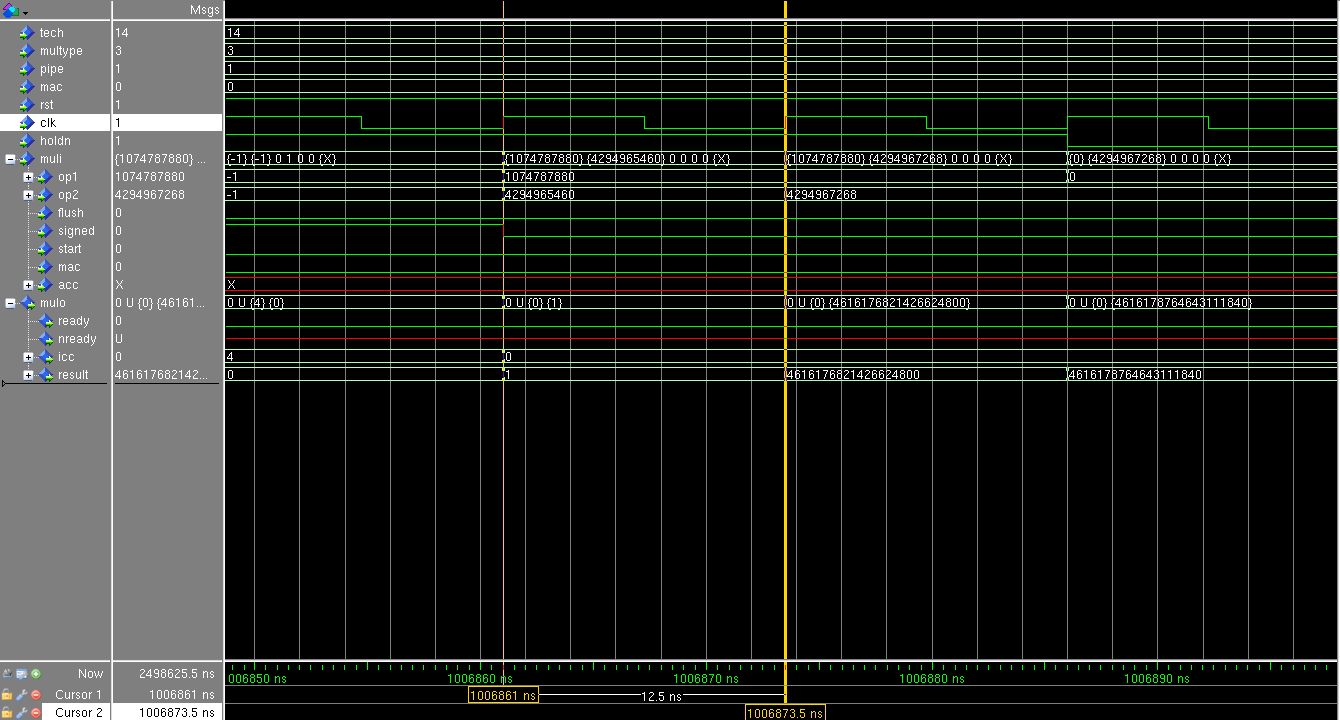
\includegraphics[width=0.45\textwidth,height=0.2\textheight,keepaspectratio]{mul32_wave.png}
\caption{Screenshot of the Modelsim's Wave for the multiplier. For this particular simulation a 16x16 operation is shown, along with all the appropriate signals.}
\label{fig:mul32_wave}
\end{figure}

Notice that the value ``P/f'' indicate the energetic efficiency of the processor, since the power
consumption is almost proportional to the clock frequency we can use this value to estimate the
power consumption at different clock frequencies.

From the synthesis report we can also see the slowest path which determines the max clock
frequency.

This path is from ``ddrsp0.ddrc0/ddr\_phy0/ddr\_phy0/xc4v.ddr\_phy0/ddgen[24].gi/FF1'' to
``ddrsp0.ddrc0/ddr32.ddrc/read\_buff/xc2v.x0/a0.x0/Mram\_rfd1''

Those components belong to the SDRAM controller and the path is located between the controller
and the physical interface with the memory.

The synthesis of our modified version gave us the results showed in Table 2:


\begin{figure}[H]
\centering
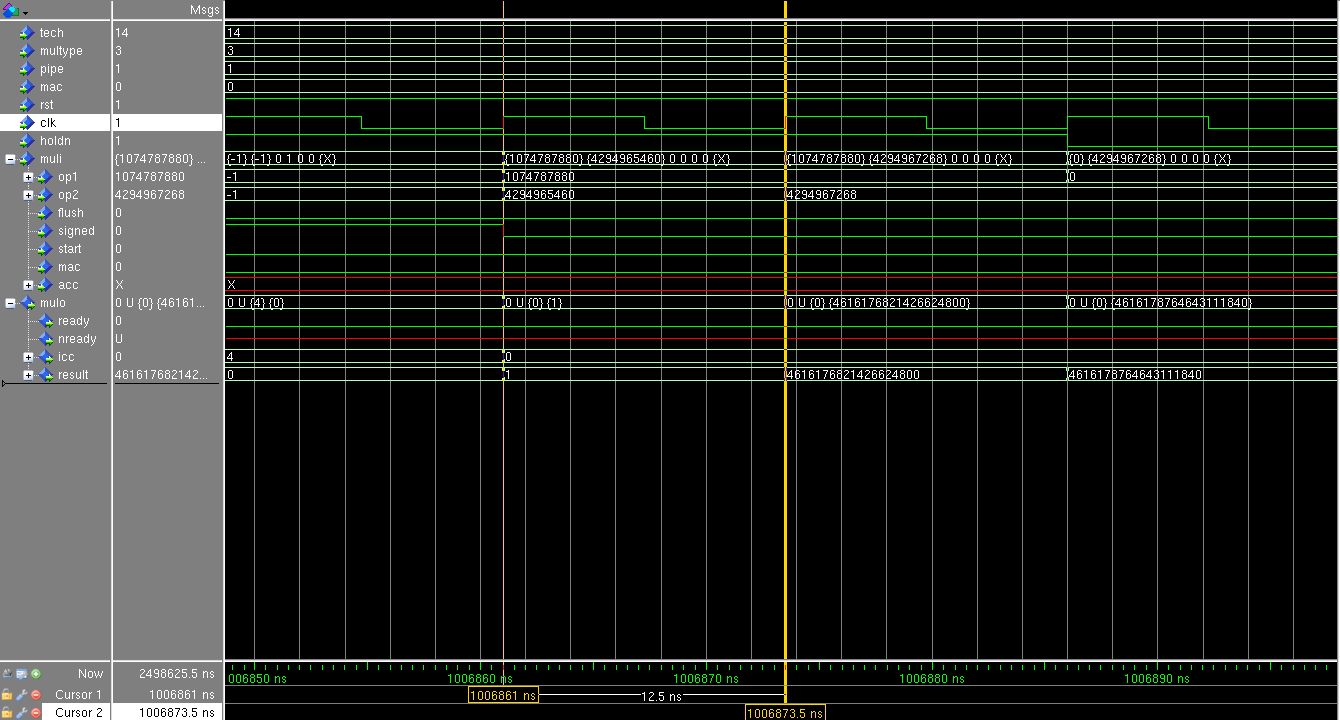
\includegraphics[width=0.45\textwidth,height=0.2\textheight,keepaspectratio]{mul32_wave.png}
\caption{Screenshot of the Modelsim's Wave for the multiplier. For this particular simulation a 16x16 operation is shown, along with all the appropriate signals.}
\label{fig:mul32_wave}
\end{figure}

As we expected the area consumption is quite worse because the unit we designed is way more
complex than the baseline, in particular the look-up table in the divider consumes lots of area.

Also the power consumption increased for the same reason, the algorithm is more complicated so
more energy is consumed to do all the calculations, but fortunately the disadvantage is negligible
compared to the advantage as it will be shown later.

The only parameter which is better is the max clock frequency achievable but probably this is only
due to the synthesis tool that rearranged the processor's component in a different way that is
better for the clock performance.

\subsection{Benchmark Scores}

Once the processor is synthesized has been loaded in a FPGA board, then Linux has been launched
on the processor as much as several benchmarks. In Table 3 the execution times of these
benchmarks are reported, for detailed scores see the excel file attached.

\begin{figure}[H]
\centering
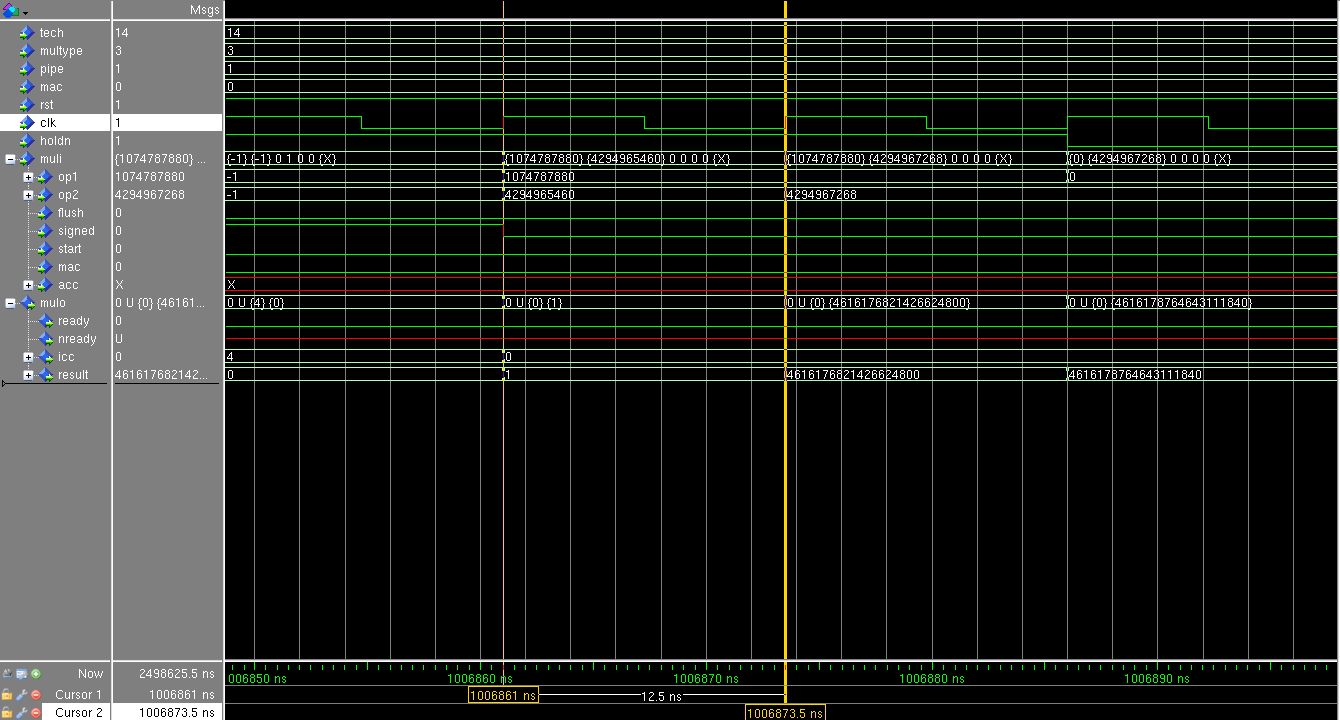
\includegraphics[width=0.45\textwidth,height=0.2\textheight,keepaspectratio]{mul32_wave.png}
\caption{Screenshot of the Modelsim's Wave for the multiplier. For this particular simulation a 16x16 operation is shown, along with all the appropriate signals.}
\label{fig:mul32_wave}
\end{figure}

The scores obtained with the modified processor are reported in Table 4.

\begin{figure}[H]
\centering
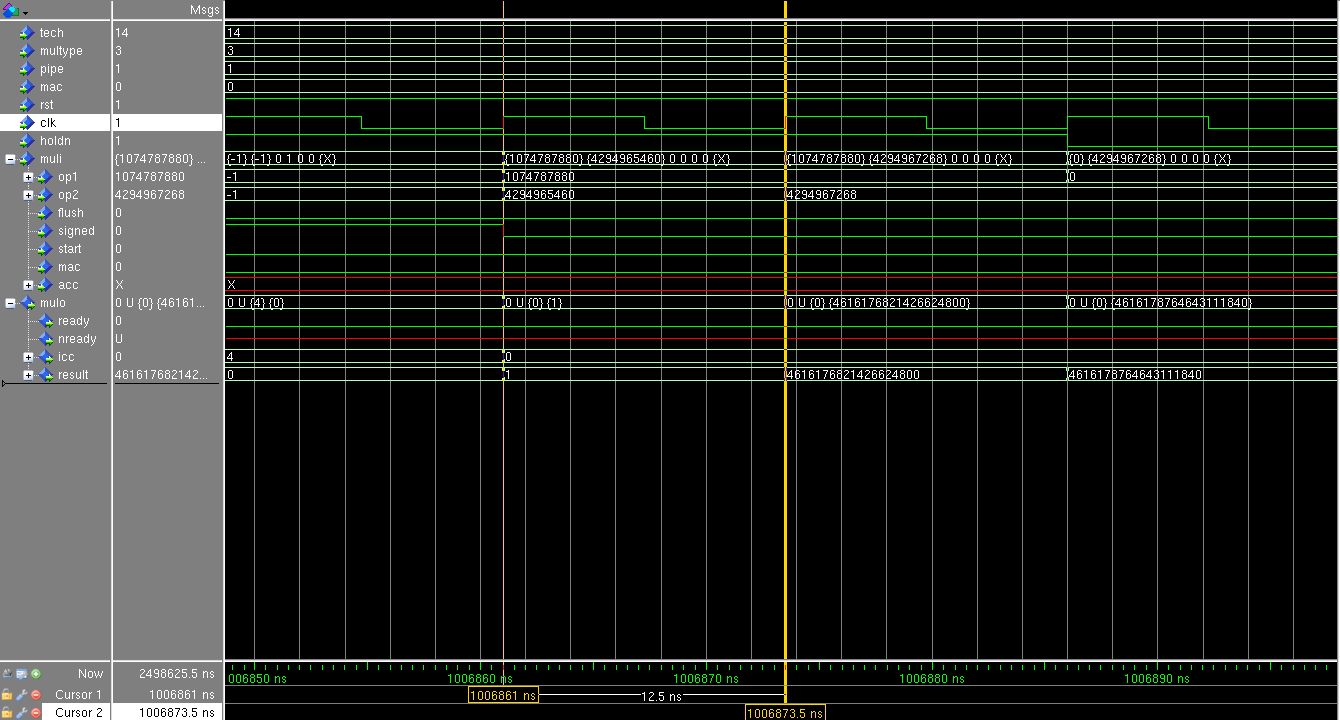
\includegraphics[width=0.45\textwidth,height=0.2\textheight,keepaspectratio]{mul32_wave.png}
\caption{Screenshot of the Modelsim's Wave for the multiplier. For this particular simulation a 16x16 operation is shown, along with all the appropriate signals.}
\label{fig:mul32_wave}
\end{figure}

From these results we can see that almost every benchmark had a slight improvement, in the end
the total execution time improved by 2.7\%.

These scores are not as good as we expected but probably the execution of an operative system
on the processor cause a not negligible overhead in the execution due to the scheduling (the
divider takes about half the time to execute but the execution time of the division related
benchmarks is only about 10\% better).

\subsection{Metrics Comparison}

In order to get a fair comparison between the baseline and the improved processor some standard
metrics have to be calculated and studied.

Usually these metrics are A, the area consumption here calculated as the weighted sum of the
number of occupied slices and the number of 4-input LUTs used where the weight is the reciprocal
of the number of available resources, D is the delay or the reciprocal of the max clock frequency
and indicate the delay of the slowest path, P is the power and it's simply calculated as the total
power consumed by the Dhrystone benchmark used for the simulation and BS is the benchmark
score which indicate how fast a program can be executed, it's calculated as the total execution
time of the benchmarks on the FPGA board.

Moreover some composite metrics can be observed: these metrics consider two or more primitive
metrics and often are more interesting than these ones because when a modification is done on
the processor usually we obtain two opposite effects, one primitive metrics increases while
another one decreases, but what we want is that all in all we have an improvement. Composite
metrics show the overall performance.

Since we want to speed-up the execution of the software while keeping the power consumption
low because this is a processor designed for embedded applications, the composite metric we are
interested the most is P*BS which show how much the processor is able to execute the software
fast with the same amount of energy.

Other composite metrics are A*D, A*BS and P*D. Since we focused on the improvement of the
execution time and power consumption one can notice that these metrics are worse in our version
compared to the baseline, because the area consumption has increased notably and the delay
hadn't had any significant changes.

Both the baseline version's and our improved version's synthesis and benchmark results have be
condensed in this metrics and their values are in the Table 5.

\begin{figure}[H]
\centering
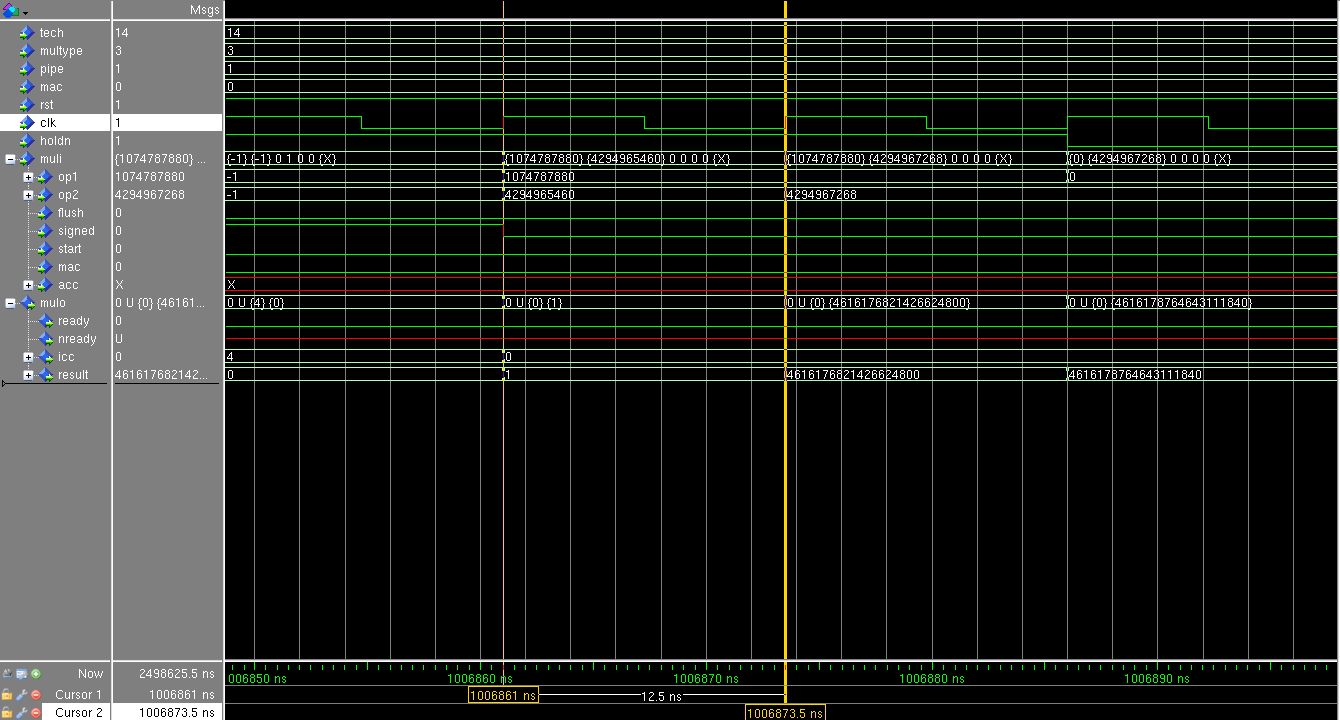
\includegraphics[width=0.45\textwidth,height=0.2\textheight,keepaspectratio]{mul32_wave.png}
\caption{Screenshot of the Modelsim's Wave for the multiplier. For this particular simulation a 16x16 operation is shown, along with all the appropriate signals.}
\label{fig:mul32_wave}
\end{figure}
